% (This file is included by thesis.tex; you do not latex it by itself.)
\chapter{Simulation Study}
\section{Data Simulation Scheme}\label{sec:sim_scheme}
Simulating network data to assess the different variable selection methods and to reproduce the experiments is vital. Data can be synthetically generated using various network simulation software tools which may require GPUs to perform large-scale simulations faster and to gain deeper insights. We present an alternative technique for simulating the TCR network data and then compute performance measures to assess the robustness, accuracy, and other parameters of the variable selection models implemented earlier. We analyze each of the network properties from the observed data, try to find any implicit relations, approximate the property distributions, and recreate the data correlation among the explanatory variables in the simulated data set. The original TCR repertoire data was heterogeneous in nature which led us to extract the summary statistics for each feature and then create an aggregated data set. Since any correlation that exists among the network features is observed in the heterogeneous (non-aggregated) form of the data, it therefore vital for us to simulate the data in the non-aggregated form and then derive the summary statistics.\par
\begin{figure}[H]
\centering
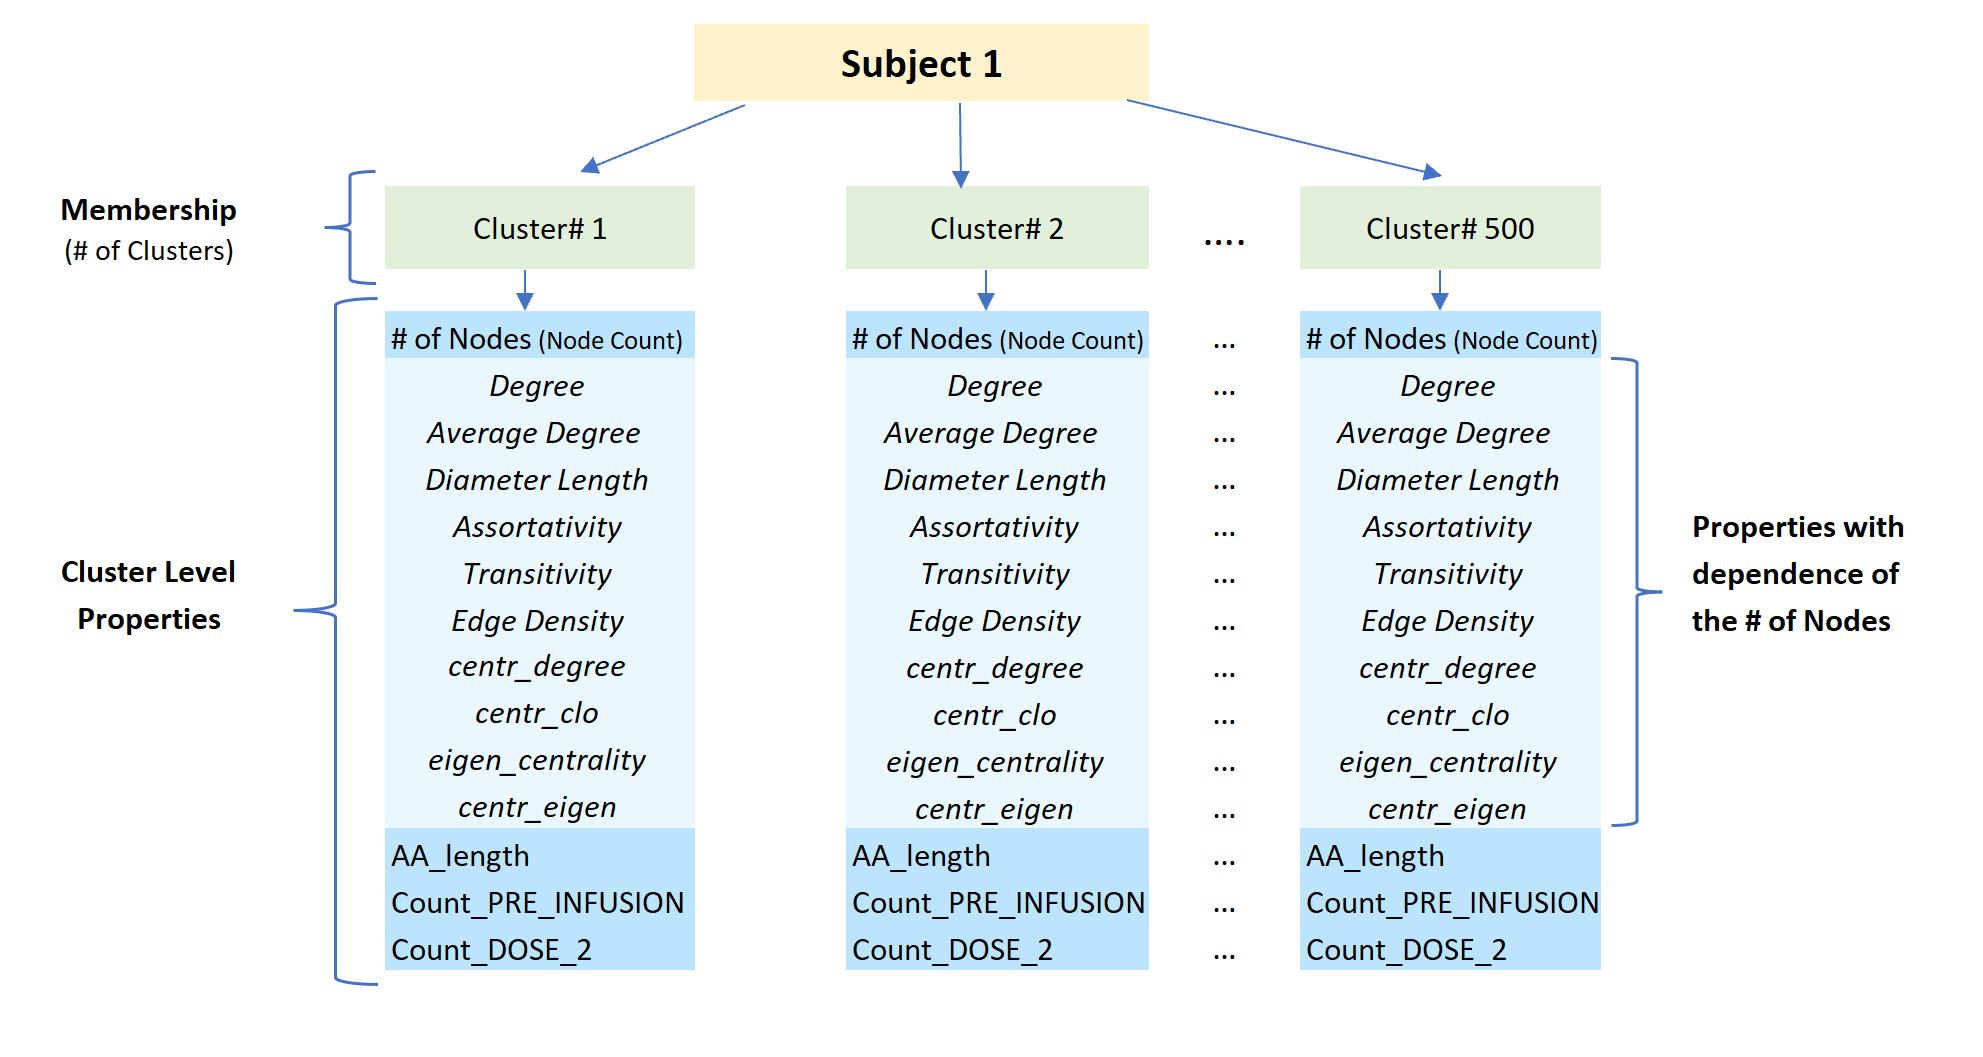
\includegraphics[scale=0.75]{Network_hierarchy.jpg}
\caption{Dependencies and Hierarchy of the Network Properties}%
{The above figure gives a general idea of how the TCR network properties are dependent on each other and a rough hierarchical structure. This information was derived by analyzing the real data.}
\label{fig:ntwrk_hier}
\end{figure}
A high-level hierarchy of the network properties as observed in the real data is shown in the \autoref{fig:ntwrk_hier}. The TCR repertoire network data of each subject has multiple clusters (membership) of varied levels of complexity. Some clusters could be dense (have more nodes), and some could be sparse (have fewer nodes). Refer \autoref{fig:cluster_ex}. Each cluster then has a varied number of nodes and associated nodal properties. As a result, simulating this network data first requires generating the clusters for a subject. Then for each cluster we simulate the \# of nodes and the associated network features.\par
\begin{figure}[H]
\centering
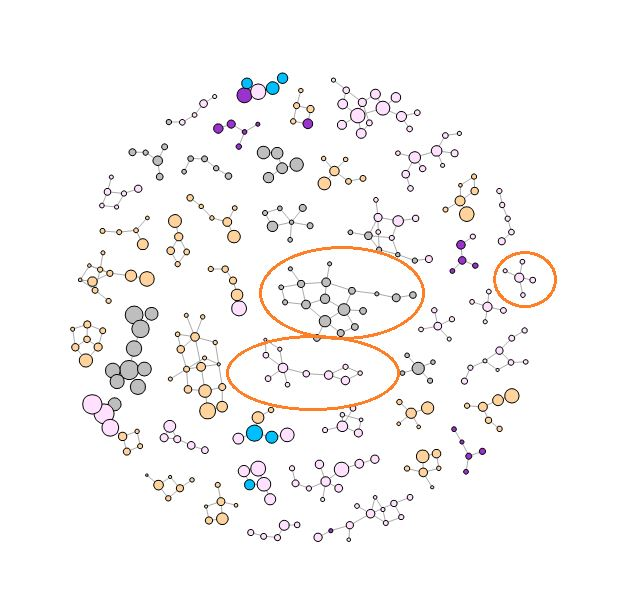
\includegraphics[scale=1]{Cluster_sample.jpg}
\caption{Sample TCR network data of a subject showing multiple clusters and nodes.}
\label{fig:cluster_ex}
\end{figure}
\subsection{Simulating Cluster-count (Membership) data}\label{subsubsec:sim_clust_cnt}
The number of clusters for each of the 65 patients were observed from the original TCR repertoire data. \autoref{fig:cluster_ex} represents the distribution of the cluster-count and the log(cluster-count) of the original TCR repertoire data. The log(cluster-count) has an approximate normal form. We then compute the mean and the standard deviation of this distribution. Using inbuilt R function, $rlnorm()$, we draw random samples from a log normal distribution, with $\text{meanlog} = \text{mean}(\log(\text{cluster-count}))$ and $\text{sdlog} = \text{sd}(\log(\text{cluster-count}))$, we generate samples which are then used as the cluster-count for 1000 dummy patients.\par
The\autoref{fig:clust_obsv_sim} represents the histogram of the cluster-count from the original observed data versus the cluster-count from the simulated data. The plots show the semblance between the original data and the simulated data. The simulated cluster-count data serves as the basis for simulating the remaining properties.\par
\begin{figure}[H]
\centering
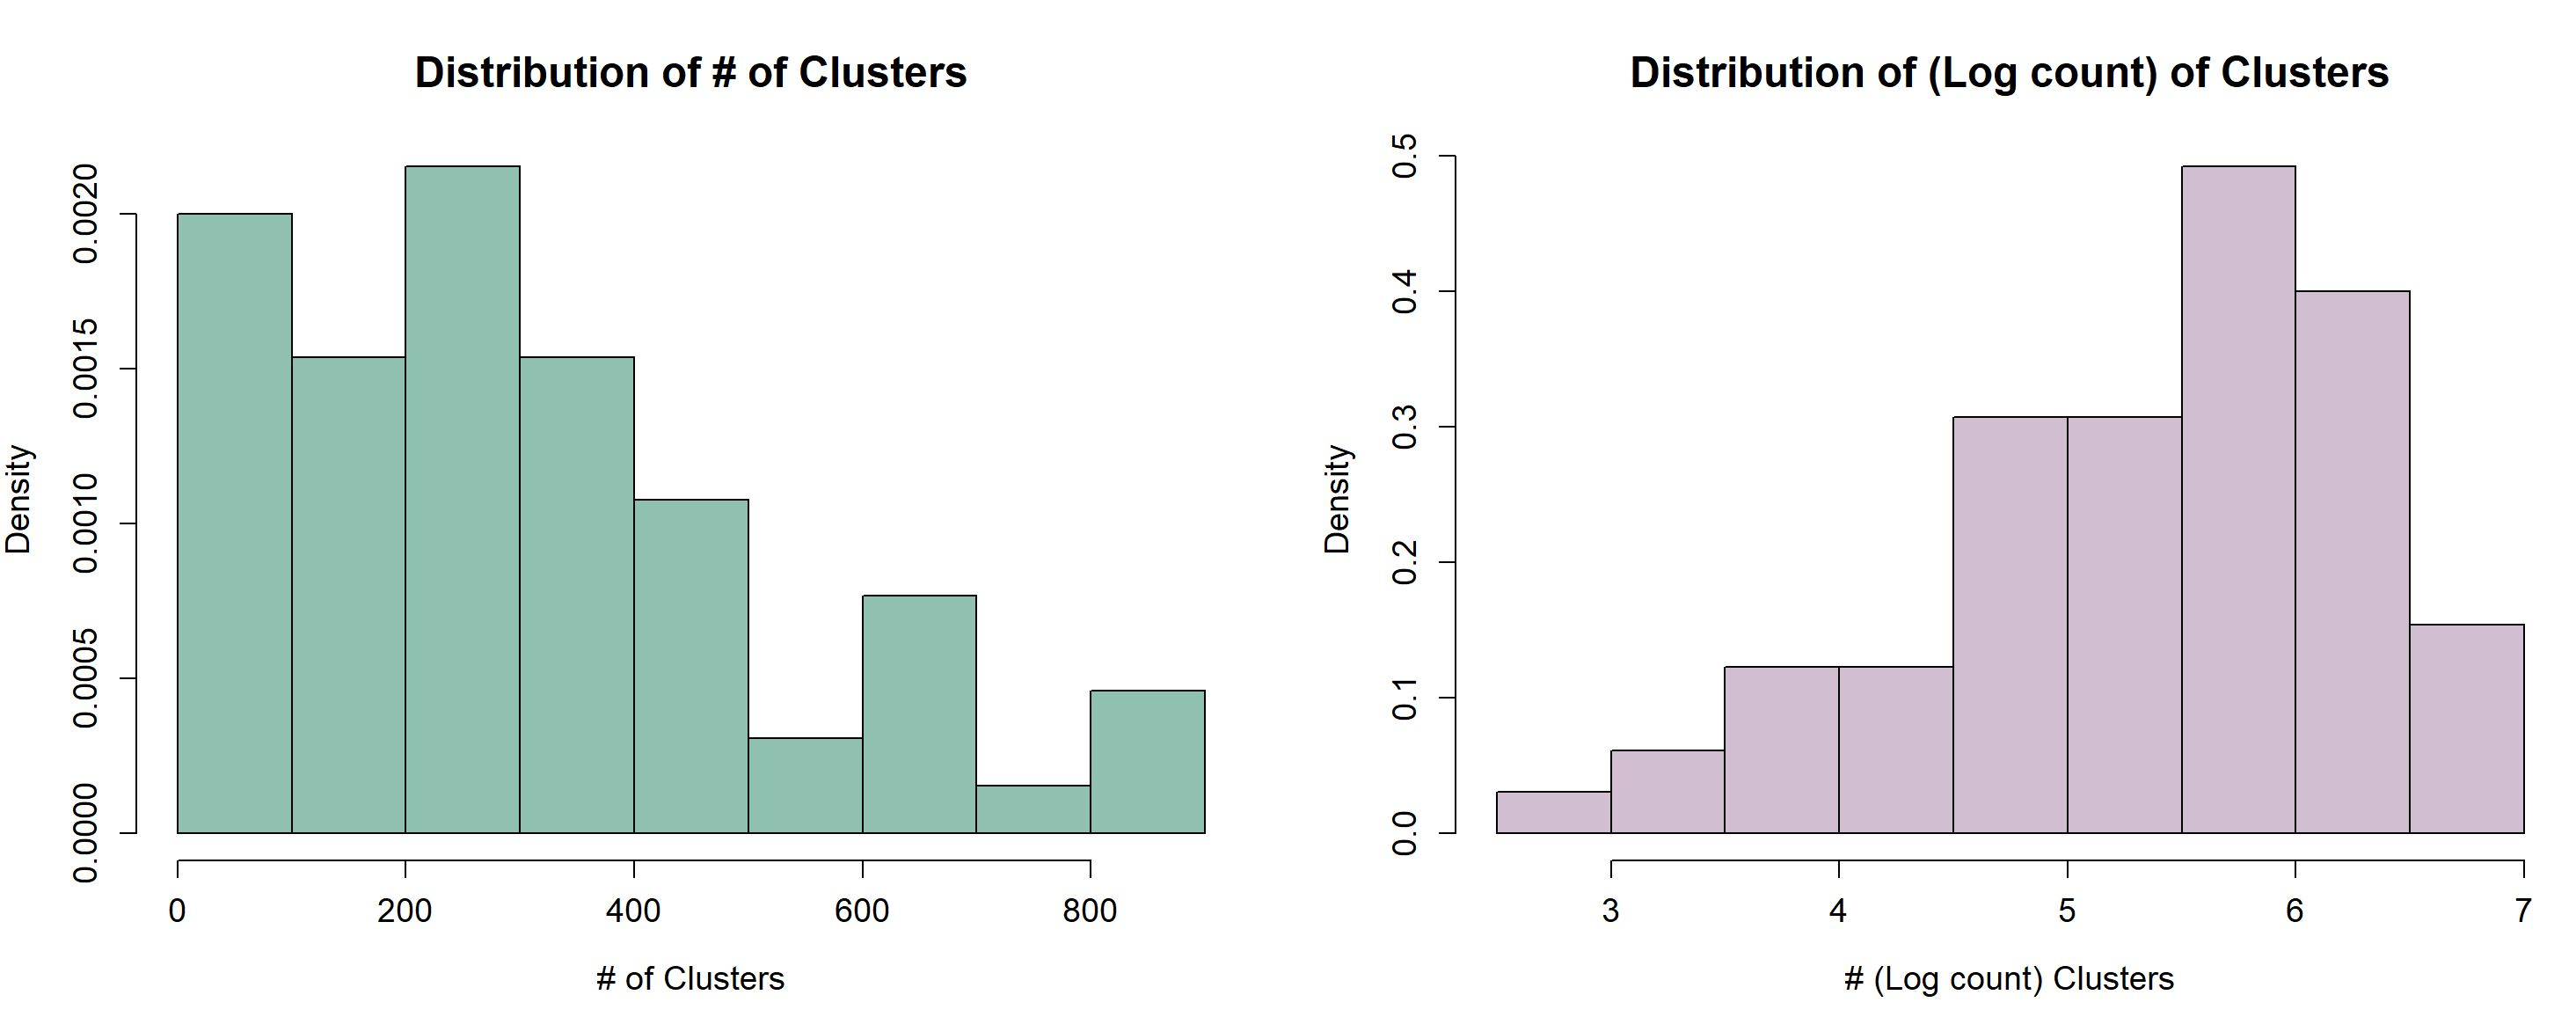
\includegraphics[scale=0.5]{Cluster_real_dt.jpg}
\caption{Histogram plot for cluster-count and log(cluster-count) of the 65 patients' TCR repertoire data.}
\label{fig:cluster_ex}
\end{figure}
\begin{figure}[H]
\centering
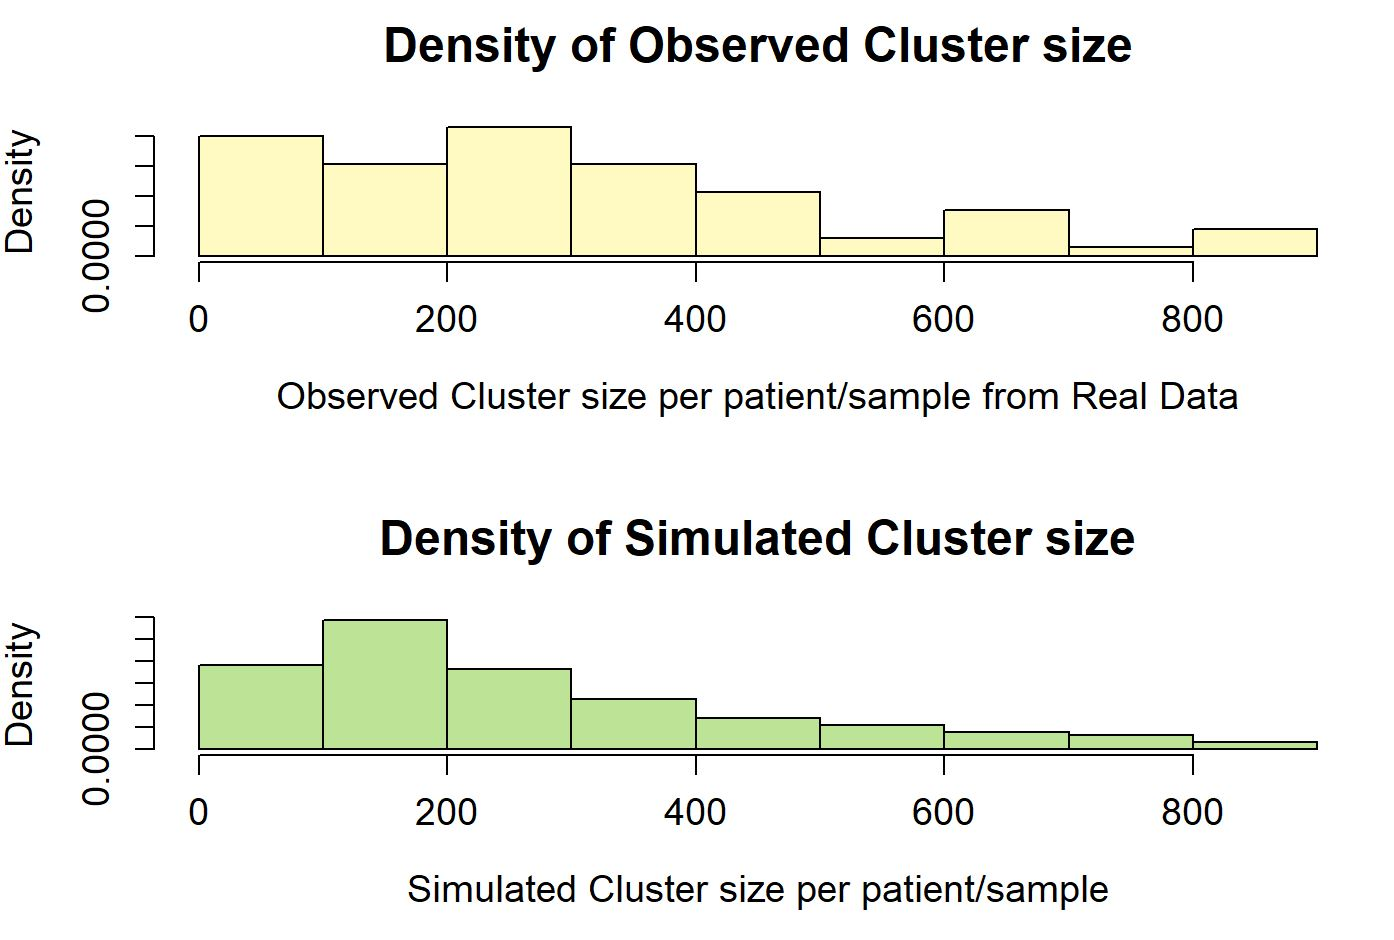
\includegraphics[scale=0.7]{Clust_obs_sim.jpg}
\caption{Histogram plots for the \lq Cluster-count' from the original data versus the \lq Cluster-count' from the simulated data.}
\label{fig:clust_obsv_sim}
\end{figure}
\subsection{Simulating Node-count data}\label{subsubsec:sim_node_cnt}
The simulated cluster-count data dictates the number of TCR network property rows that each of the 1000 dummy patients would have. We then set to simulate the node-count associated with each of the clusters. It is observed that the node-count data from the original TCR repertoire has a right-skewed distribution with maximum frequency occurring for the values 2 and 3, and the remaining subsection has an approximate log-normal form. Therefore, to simulate the node-count, the entire distribution is considered in segments. We calculated the probabilities of the node-count = 2 and 3 and simulate data for these two categories. For the remaining segment of the distribution, we draw samples from the $rlnorm()$ function using a similar technique as we did for simulating the cluster-count data. The \autoref{fig:node_count_obsv_sim} depicts the histogram of the node-count from the original observed data versus the simulated data where we can observe the similarity in the two density functions. We then derive the summary statistics for the simulated node-count data and will use the aggregated data for assessing the various models in subsequent sections.\par
\begin{figure}[H]
\centering
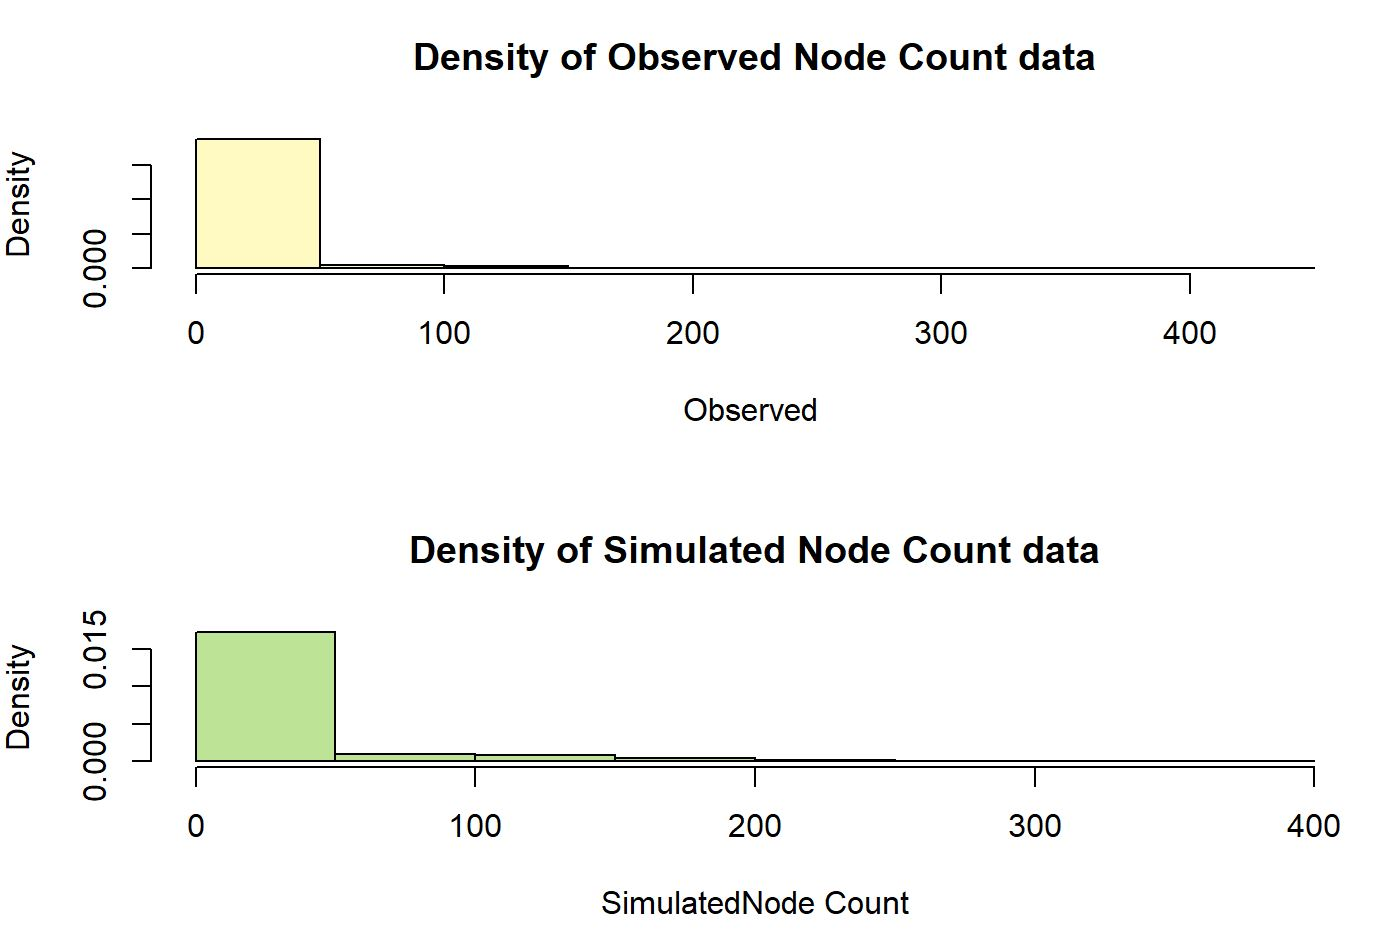
\includegraphics[scale=0.75]{Node_count_obs_sim.jpg}
\caption{Histogram plots for \lq Node-count' from the original data versus the \lq Node-count' from the simulated data.}
\label{fig:node_count_obsv_sim}
\end{figure}

\subsection{Simulating Remaining Network Properties} \label{subsubsection:sim_rem}
After the node-count data is simulated, the remaining set of network properties can be simulated. It is observed that some of the properties have a distinct value for certain values of Node-count. The \autoref{tab:node_depnd} outlines some of these relations. Probabilities of the node-count values = 2 and 3 evaluated in the \nameref{subsubsec:sim_node_cnt} sub-section are used to simulate the data for the remaining network properties. Following this, the simulated row-wise data is aggregated for each of the network properties, resulting in a single row of data per dummy patient. \autoref{fig:assort_obsv_sim} represents the histogram comparison of the observed versus simulated data of the network property called \lq Assortativity'.\par
\begin{table}[H]\centering
\caption{Dependency of some TCR properties on the Node\_count}
\begin{tabular}{|c|c|c|}\hline
\cellcolor[HTML]{D9E1F2}\textbf{TCR properties} & \cellcolor[HTML]{D9E1F2}\textbf{Values}  & \cellcolor[HTML]{D9E1F2}\textbf{Values} \\ \hline
\cellcolor[HTML]{EAEAEA}Node\_count  & \cellcolor[HTML]{EAEAEA}2 & \cellcolor[HTML]{EAEAEA}3 \\ \hline
Assortativity  & NA & -1 ($99.7\%$ times) \\ 
Transitivity  & NA & - \\ 
Degree  & 1 & - \\ 
Diam\_length  & 2 & - \\
Deg\_avg  & 1 & - \\ 
Edge\_density  & 1 & - \\ 
Centr\_degree  & 0 &  -\\ 
Centr\_clo  & NA & - \\ 
Eigen\_centrality  & 1 & - \\ 
Centr\_eigen  & NA & -\\ \hline
\end{tabular}
\label{tab:node_depnd}
\end{table}
\begin{figure}[H]
\centering
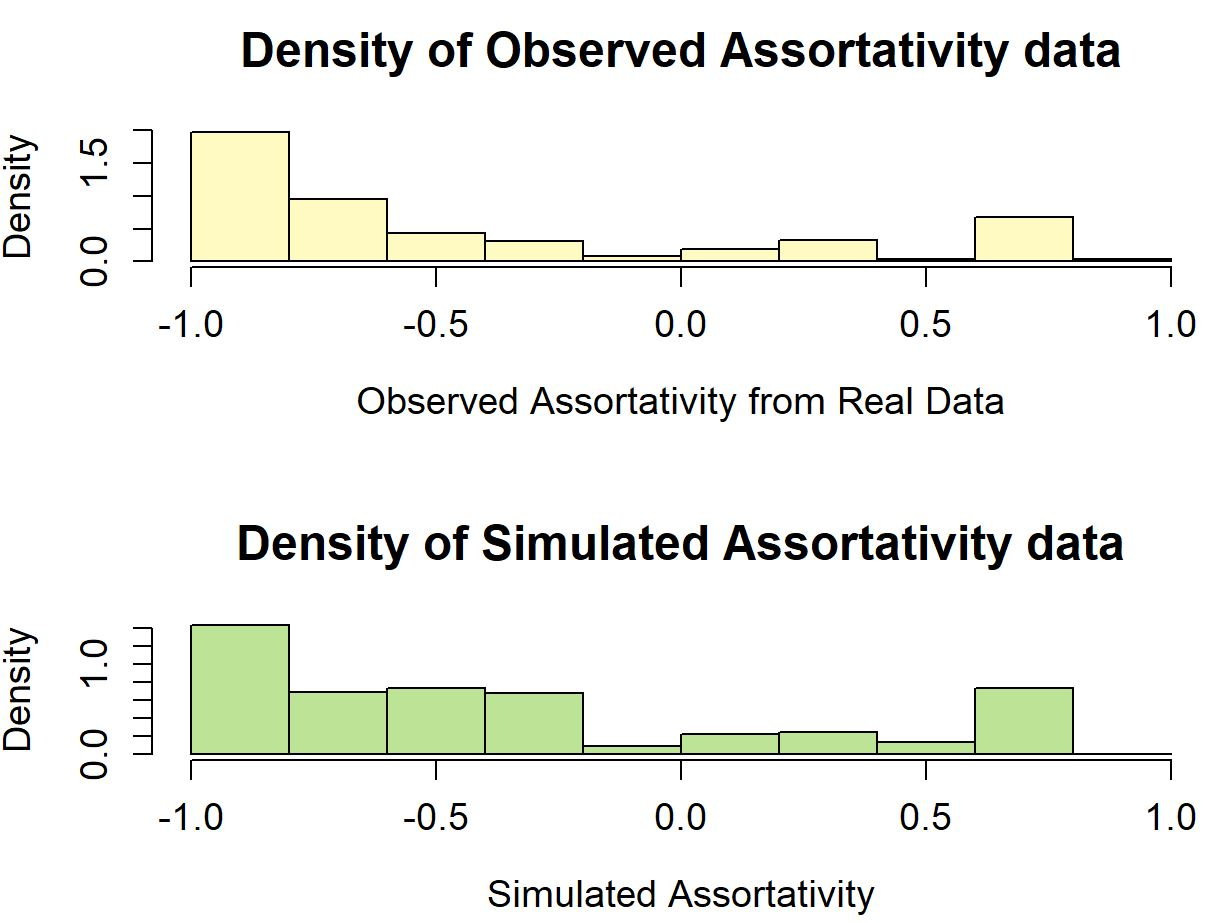
\includegraphics[scale=0.75]{Assort_obs_sim.jpg}
\caption{Histogram plots for comparing the density of \lq Assortativity' from the observed data and from the simulated data.}
\label{fig:assort_obsv_sim}
\end{figure}

\subsection{Simulating Response Variable} \label{subsubsec:simresponse}
In order to simulate the response variable, while keeping the correlation between the explanatory variables and the response intact, we use the model from the sub-section \nameref{subsec:plasso_cv}. In a binary classification setting with response variable $y_i \in{0,1}$ assume that we have independent and identically distributed observations $(\mathbf{x}_i, y_i)$ where $i=1, . . . , n$ of a $p$-dimensional vector $\mathbf{x}_i \in \mathbb{R}^p$. The log of odds is given as:
\begin{equation*}
\begin{split}
\log\{\frac{p_{\pmb{\beta}}(\mathbf{x}_i)}{1-p_{\pmb{\beta}}(\mathbf{x}_i)}\}=\beta_0+\beta_1X_1+..+\beta_pX_p=\eta_{\pmb{\beta}}(\mathbf{x}_i)
\end{split}
\end{equation*}
where $p_{\pmb{\beta}} = \mathbb{P}_{\pmb{\beta}}(y_i=1|\mathbf{x}_i)$ and $\pmb{\beta}=(\beta_0,\beta_1, .., \beta_p)^T$ are the coefficients for the $p$ predictors.\par
Using the Lasso model from \autoref{subsec:plasso_cv} where we obtained feature indexes [25, 43, 82, 89] as the significant variables. We use these as the true causal variables $X_1,...,X_4$ for simulating the response variable $y_i$'s where $i\in 1,..,1000$. The log of odds $\eta_{\pmb{\beta}}(\mathbf{x}_i)$ and $p_{\pmb{\beta}}=\mathbb{P}_{\pmb{\beta}}(y_i=1|\mathbf{x}_i)$ can be written as:
\begin{equation}\label{eq:9}
\eta_{\pmb{\beta}}(\mathbf{x}_i)=\beta_0+\beta_1X_1+..+\beta_4X_4
\end{equation}
\begin{equation}\label{eq:10}
p_{\pmb{\beta}} = \mathbb{P}_{\pmb{\beta}}(y_i=1|\mathbf{x}_i) =  \frac{\exp(\eta_{\pmb{\beta}}(\mathbf{x}_i))}{1+\exp(\eta_{\pmb{\beta}}(\mathbf{x}_i))}
\end{equation}
where the $\pmb{\beta}$ coefficients are artificially created. We then sample randomly from a Bernoulli distribution using the function $rbern()$ such that 1000 random samples are generated with probability $=p_{\pmb{\beta}}$. These random samples are then used as simulated response values for our study.\par

\section{Simulation Results}\label{sec:simresults}
The simulated network property data is aggregated to produce summary statistics for each subject and is indexed like what was done for the original data. The simulated data also consists of 89 network features (individual summary statistics) and 15 network properties (feature blocks deduced by aggregating the summary statistics). The data set is then down-sampled to accommodate for the data imbalance. We assess the Lasso\_CV, Plasso, Group Lasso\_CV, Group Plasso, and Exclusive Lasso models using the simulated data. Performance measures are computed by iteratively running the variable selection models on the simulated data.\par

\subsection{Evaluation Criteria} \label{subsec:evalcrt}
We used the following measures - Sensitivity, False Discovery Rate (FDR), F1 score, Power, and Stability to evaluate the
performances of the different variable selection models. A false-positive finding means the selection of any predictor variable except the causal variables by the feature selection method. Sensitivity is defined as the proportion of correctly identifying causal variables among all causal variables in a single iteration. FDR is defined as the frequency of false-positive findings among all variables selected per method and
iteration. F-1 score is the harmonic mean of the sensitivity and (1-FDR). It is a measure of performance accuracy of the model. The power of each causal variable is calculated as the frequency of correct selections among all iterations. To estimate stability of a variable selection model, all pairwise combinations of the selected variables list from each iteration are considered. For each pair, the stability of the two lists of selected variables is determined using the Jaccard’s index given as: $J(A_i,A_j)=\frac{|A_i\cap A_j|}{|A_i\cup A_j|}$, where $A_i$ is the list of variables selected in the $i^{\text{th}}$ iteration and $A_j$ is the list of variables selected in the $j^{\text{th}}$ iteration such that $i\ne j$ and $i,j\in 1,2,..,I (\text{ total number of iterations})$. Jaccard's index, $J(A_i,A_j)=0$ if the two lists do not overlap, and $J(A_i,A_j)=1$ if the two lists contain the same variables. The average of all pairs is used as the stability value for that method.

\subsection{Simulation Results from Group Lasso\_CV and Group Plasso} \label{subsec:simstudy_grplasso}
The assessment of the Group Lasso\_CV and the Group Plasso models on the simulated data is done using the true causal variables derived using the Lasso\_CV model (refer \autoref{subsec:plasso_cv}) on the original data, as the \lq gold-standard'. The causal network properties (feature blocks) that correspond to the top network features are derived from \autoref{subsec:plasso_cv}. The performance measures for the simulation study on Group Lasso\_CV and Group Plasso models are shown in the \autoref{tab:grp_lasso_vs_lasso_sim_study}. It is observed that both Group Lasso\_CV and Group Plasso models have high sensitivity which is desirable. The FDR value for the Group Plasso model is lower than that of the Group Lasso\_CV model which is as expected. The Group Plasso model however has a much higher stability than the Group Lasso\_CV model.\\

\begin{table}[H]
\caption{Performance measures of Group Lasso\_CV and Group Plasso models.}
\resizebox{\textwidth}{!}{%
\begin{tabular}{|c|c|c|c|c|c|c|}\hline
\cellcolor[HTML]{D9E1F2}\textbf{Models} & 
\cellcolor[HTML]{D9E1F2}\textbf{True Group Indexes}  & 
\cellcolor[HTML]{D9E1F2}\textbf{Sensitivity} & 
\cellcolor[HTML]{D9E1F2}\textbf{FDR} &
\cellcolor[HTML]{D9E1F2}\textbf{F1} &
\cellcolor[HTML]{D9E1F2}\textbf{Power} &
\cellcolor[HTML]{D9E1F2}\textbf{Stability} \\ \hline
Group Lasso\_CV & Group - 5, 8, 14, 15   & 0.775 & 0.5324 & 0.5597 & 0.8, 1.0, 0.8, 0.5 &  0.5911\\ \hline
Group Plasso & Group - 5, 8, 14, 15 & 0.7 & 0.45297 & 0.6094 & 1.0, 1.0, 0.7, 0.1 & 0.8123 \\ \hline
\end{tabular}}
\label{tab:grp_lasso_vs_lasso_sim_study}
\end{table}

\subsection{Simulation Results from Lasso\_CV and Plasso} \label{subsec:simstudy_plasso}
Consider the top network features derived from the Lasso\_CV model (refer \autoref{subsec:plasso_cv}) as the \lq gold-standard' for the causal variables. The Lasso\_CV and the Plasso models are assessed using these true causal variables. It is observed that the Plasso model outperforms the Lasso\_CV model in terms of the FDR and F1 score. The remaining performance measures are at par. Refer \autoref{tab:lasso_sim_study}.\\ 
\begin{table}[H]
\caption{Performance measures of Lasso\_CV and Plasso models.}
\resizebox{\textwidth}{!}{%
\begin{tabular}{|c|c|c|c|c|c|c|}\hline
\cellcolor[HTML]{D9E1F2}\textbf{Models} & 
\cellcolor[HTML]{D9E1F2}\textbf{True Feature Indexes}  & 
\cellcolor[HTML]{D9E1F2}\textbf{Sensitivity} & 
\cellcolor[HTML]{D9E1F2}\textbf{FDR} &
\cellcolor[HTML]{D9E1F2}\textbf{F1} &
\cellcolor[HTML]{D9E1F2}\textbf{Power} &
\cellcolor[HTML]{D9E1F2}\textbf{Stability} \\ \hline
Lasso\_CV & 25, 43, 82, 89 & 1 & 0.5065 & 0.6594 & 1.0, 1.0, 1.0, 1.0 & 0.9212 \\ \hline
Plasso &  25, 43, 82, 89 & 1 & 0.2533 & 0.8533 & 1.0, 1.0, 1.0, 1.0 & 0.9111\\ \hline
\end{tabular}}
\label{tab:lasso_sim_study}
\end{table}

\subsection{Simulation Results from Exclusive Lasso\_CV} \label{subsec:simstudy_exclusvlasso}
For assessing the Exclusive Lasso model on the simulated data we use the top network features, derived using the Lasso\_CV model (refer \autoref{subsec:plasso_cv}), as the \lq gold-standard' for the causal variables. It is observed that Exclusive Lasso consistently identifies the true causal variables in every iteration and therefore has a perfect sensitivity value. This result asserts the findings from the Lasso models. Note that Exclusive Lasso shows a very high FDR and low F1 values. This observation is due to the compulsion of the Exclusive Lasso model to select at least one feature from each of the feature blocks. \\[4pt]
\begin{table}[H]
\caption{Performance measures of Exclusive Lasso model.}
\resizebox{\textwidth}{!}{%
\begin{tabular}{|c|c|c|c|c|c|c|}\hline
\cellcolor[HTML]{D9E1F2}\textbf{Models} & 
\cellcolor[HTML]{D9E1F2}\textbf{True Feature Indexes}  & 
\cellcolor[HTML]{D9E1F2}\textbf{Sensitivity} & 
\cellcolor[HTML]{D9E1F2}\textbf{FDR} &
\cellcolor[HTML]{D9E1F2}\textbf{F1} &
\cellcolor[HTML]{D9E1F2}\textbf{Power} &
\cellcolor[HTML]{D9E1F2}\textbf{Stability} \\ \hline
Exclusive Lasso\_CV & 25, 43, 82, 89 & 1 & 0.8 & 0.3333 & 1, 1, 1, 1 & 1 \\ \hline
\end{tabular}}
\label{tab:exclusv_lasso_sim_study}
\end{table}